\chapter{Projekt}
\thispagestyle{chapterBeginStyle}
W danym rodziale opisana została aplikacja pod względem technicznym. 

\section{Opis systemu}
Tworzenie aplikacji internetowej to skomplikowany proces, który może przysporzyć wiele problemów w przyszłości. Pierwszym problemem jest utrzymanie istniejącego kodu, to znaczy kontrolowanie stanu aplikacji i naprawianie pojawiających się błędów, związanych z pierwotną implementacją. Drugim problemem jest możliwość rozwoju aplikacji, w momencie w którym aplikacja przynosi zyski i sprawdza się w kontakcie z użytkownikiem, oczywistym podejściem jest rozbudowa aplikacji. W tym celu podczas planowania implementacji trzeba zastanowić się nad odpowiednim podejściem. W tym celu powstały wzorce projektowe, które pomagają programistom uporać się z różnymi problemami w sposób zorganizowany, zoptymalizowany ułatwiając problemy podczas implementacji, zwiększając czytelność kodu. 

\section{Wzorzec Architektoniczny Model-View-Controller}
System zbudowany został w oparciu o model MVC, czyli Model-View-Controller.
Jest to podejście architektoniczne, które dzieli aplikacje na trzy główne komponenty.
Model, odpowiedzialny za dostęp i przechowywanie danych. View, czyli widok odpowiada za interfejs użytkownika, jak dane są przedstawiane i odbierane. Controller zajmuje się logiką biznesową komunikując się z modelem i widokiem. Widok dostarcza informacje od klienta, które obsługiwane są przez Controller i odpowiednie zmiany wprowadzane są do modelu. 

\begin{figure}[h]

	\centering
		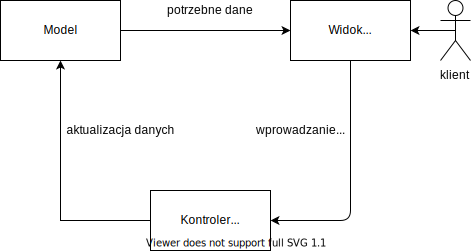
\includegraphics[width=1.00\textwidth]{mvc-diagram}		
		\caption{Komunikacja pomiędzy komponentami we wzorcu MVC }
\end{figure}

Zalety korzystania z wzorca MVC to lepsza przejrzystość kodu, skalowalność i utrzymanie. W
momencie wystąpienia błędu, może zostać obarczona odpowiedzialnością jedna z trzech części
systemu, więc optymalizuje to znacząco proces szukania miejsca, w którym dany błąd
występuje.  

\section{Wymagania funkcjonalne i niefunkcjonalne}
\paragraph{Wymagania funkcjonalne}
\begin{enumerate}
	\item Przegląd listy użytkowników
	\item Przegląd listy zadań 
	\item Tworzenie, edytowanie, usuwanie zadań
	\item Korzystanie z Tablicy Kanban w celu raportowania postępów w zadaniach
	\item Wyświetlanie Statystyk projektu w postaci wykresów
	\item Podstawowa autentykacja użytkownika
	\item wyświetlanie szczegółów związanych z danym zadaniem. Szczegółowe parametry zadania to:
	\begin{enumerate}[leftmargin=3em]
		\item nazwa,
		\item data do zakończenia zadania,
		\item użytkownik przypisany do zadania, 
		\item kolumna w której aktualnie znajduje się dane zadanie,
		\item opis zadania
		\item sekcja komentarzy
		\item nazwa użytkownika tworzącego zadanie
	\end{enumerate}
\end{enumerate}
\paragraph{Wymagania funkcjonalne dodatkowe dla administratora}

		\begin{enumerate} 
		\item tworzenie, aktywacja kont użytkowników, dostęp do większej ilości danych w porównaniu do użytkownika
		\item ustawienie czasu po jakim czyszczona jest historia czynności związanych z zadaniami 
		\item Konfiguracja tablicy:
	\begin{enumerate}[leftmargin=3em]
			\item określenie nazwy tablicy i kolumn
			\item określenie liczby kolumn, 
			\item wybranie domyślnej kolumny (na którą wprowadzane będą nowe zadania)
			\item wybranie końcowej kolumny (kolumna,która automatycznie zmienia status zadania na skończony), Opcjonalne
		\end{enumerate}

\end{enumerate}
\paragraph{Wymagania niefunkcjonalne}
\begin{enumerate}
	\item możliwość użytkowania systemu po godzinnym szkoleniu
	\item komunikacja z bazą dancyh nie dłuższa niż 200ms na każde zapytanie 
	\item aplikacja responsywna, aby nie było problemu wykonywać wszystkie założenia funkcjonalne na urządzeniu mobilnym
\end{enumerate}


\section{Diagram pakietów}





\section{Projekt bazy danych}

Sekcja ta w pełni skupiona jest na budowie bazy danych. Najpierw zdefiniowane zostały dane potrzebne do przechowywania.
Pierwszym rodzajem danych jest Tablica (tabela board), która przetrzymuje informacje o tablicy, z ilu  składa się kolumn, która kolumna jest kolumną domyslna, a która zamykającą zadania.
Kolejnym typem potrzebnym do przechowywania będzie wyżej wspomniana kolumna, która przechowuje status nazwę, kolejnosć wyswietlania na tablicy. Kolejnym typem jest Użytkownik, to jedna z najbardziej skomplikowanych tabel w całej bazie, ponieważ jest ona w relacji z zadaniami, które stworzył (mapowane poprzez pole ownedBy), w relacji z zadaniami do których jest aktualnie przypisany (pole assignedTo). Tabela z użytkownikami przetrzmuje informacje dotyczące korzystania z aplikacji i te  pozwalające autoryzować sesję po stronie klienta. Posiada również relacje z tabelą authority, która znowu odpowiedzialna jest za nadawnianie odpowiednich uprawnień do korzystania z aplikacji. Ostatnim z ważniejszych typów danych jest Zadanie i Komentarz. Zadanie jest to typ opisujący jak tylko może zadanie, przechowuje status w zależnosci od kolumny w której zadanie się znajduje, użytkowników powiązanych z utworzeniem zadania/ pracą nad zadaniem, a ostatnim typem będzie komentarz czyli tabela przetrzymująca komentarze odnoszące się do różnych zadań.

Jako serwer bazy danych wykorzystany został MySql serwer jako że jest to ....
W celu kontroli wersji projektu bazy danych do serwera podpięta jest biblioteka zwana Liquibase, która przechowuje wszystkie skrypty związane z tworzeniem bazy danych, modyfikacją tabel lub danych w formacie XML. Liquibase pomaga wprowadzać zmiany na istniejącej bazie danych przy zachowaniu poprzedniego stanu, zostawiając po udanej modyfikacji historię zmian. 

\section{Przypadki użycia}

W tym podrozdziale przedstawione zostały najważniejsze przypadki użycia aplikacji.


\begin{table}[h!]

\begin{tabular}{ |p{2cm}||p{13cm}|  }
	
	\hline
	\multicolumn{2}{|c|}{Rejestracja nowego użytkownika} \\
	\hline
	Aktorzy: &klient , serwer autoryzacyjny administrator\\
	\hline
	Warunki wstępne: & sesja klienta nie jest autoryzowana\\ 
	\hline
	Scenariusz: &
	\begin{enumerate}[leftmargin=0em]
		\item klient wchodzi na panel rejestracji za pomocą linka "Create Account" lub używając przycisku na nagłówku strony 
		
		\item po wypełnieniu przez klienta formularzu rejestracyjnego zachodzi proces walidacji danych

		\item  gdy walidacja przeszła pomyślnie: system wyświetla komunikat o sukcesie rejestracji i informuje,że potrzebna jest jeszcze aktywacja konta

	\begin{enumerate}[leftmargin=2em]
	 	\item  System zapisuje dane na bazie, hasło zostaje zakodowane.
	 		
	 		\item  System generuje losowy 8-cyfrowy klucz aktywacyjny dla użytkownika i wysyła na podany w formularzu e-mail link aktywacyjny.
	 		
	 		\item Klient  aktywuje konto za pomocą linka, który otrzymał na skrzynkę pocztową e-mail.
	\end{enumerate}
		
		\item  gdy walidacja zauważyła błędy w formularzu: wyświetla się komunikat błędu, zaznaczone zostają błędne pola
			\end{enumerate}
\\
	\hline

\end{tabular}

	\caption{Przypadek użycia - rejestracja nowego użytkownika}
\end{table}

\begin{table}[h!]
\begin{tabular}{ |p{2cm}||p{13cm}|  }
	
	\hline
	\multicolumn{2}{|c|}{Logowaniea} \\
	\hline
Aktorzy: &klient , serwer autoryzacyjny, system prezentujący\\
	\hline
Warunki wstępne: & sesja klienta nie jest autoryzowana, klient posiada aktywne konto\\
	\hline
	Scenariusz: &
	\begin{enumerate}
		\item klient wchodzi na panel logowania za pomocą linka "Log int" lub używając przycisku na nagłówku strony 
		\item klient wprowadza prawidłowe dane, nie zaznacza pola 'remember me'
		\begin{enumerate}
			\item system sprawdza czy istnieje użytkownik o podanych informacjach kwalifikujących
			\item system autoryzacyjny odnajduje w bazie użytkownika,
			\item system wysyła do systemu prezentującego wiadomość o poprawnym procesie weryfikacji, więc użytkownik zostaje przekierowany do widoku głównego po udanym logowaniu i przyznawane są prawa do przeglądania stron odpowiednich dla roli użytkownika, czyli ROLE\_ADMIN lub ROLE\_USER
		\end{enumerate}
		\item klient wprowadza prawidłowe dane,  zaznacza pole 'remember me'	
		\begin{enumerate}
			\item system autoryzacyjny odnajduje w bazie użytkownika,
			\item system autoryzacyjny tworzy 20-cyfrowy unikalny kod zwany tokenem i umieszcza go dla danego użytkownika
			\item system wysyła do systemu prezentującego wiadomość o poprawnym procesie weryfikacji, więc użytkownik zostaje przekierowany do widoku głównego po udanym logowaniu i przyznawane są prawa do przeglądania stron odpowiednich dla roli użytkownika, czyli ROLE\_ADMIN lub ROLE\_USER
		\end{enumerate}
		\item klient wprowadza złe dane
		\begin{enumerate}
			\item	system nie odnajduje użytkownika o podanych informacjach kwalifikujących , komunikuje się z systemem prezentującym o braku podanego użytkownika
			\item  system prezentujący wyświetla komunikat o prawdopodobnie źle wpisanym loginie lub haśle.
		\end{enumerate}
	\end{enumerate}
	\\
	\hline

\end{tabular}
	\caption{Przypadek użycia - Logowanie}
\end{table}


\begin{table}[h!]
\begin{tabular}{ |p{2cm}||p{13cm}|  }
	
	\hline
	\multicolumn{2}{|c|}{Dodawanie Zadania} \\
	\hline
Aktorzy: &użytkownik, serwer prezentujący, serwer obsługujący bazę danych\\
	\hline
Warunki wstępne: &sesja użytkownika jest autoryzowana i jest on na stronie "Board" lub "Task List"\\
	\hline
	Scenariusz: &

\begin{enumerate}
	\item Użytkownik przechodzi do panelu tworzenia nowego zadania po wciśnięciu przycisku "Create Task" zarówno na stronie "Board" jak i "Tasks List"
	\item pojawia się formularz z informacjami do podania na temat zadania, niektóre niezbędne do stworzenia zadania, niektóre opcjonalne
	\item po ukończeniu wypełniania formularza i kliknięciu przycisku "OK" system waliduje poprawność otrzymanych danych:
	\begin{enumerate}
		\item gdy dane odnośnie zadania zgadzają się, użytkownik przekierowywany jest na stronę, z której otworzył panel tworzenia zadania
		\item gdy dane odnośnie zadania nie zgadzają się, panel prezenetujący wyświetla pola z błędnymi informacjami
		\item użytkownik może poprawić dane i próbować stworzyć zadanie ponownie
	\end{enumerate}
\end{enumerate}\\
\hline
\end{tabular}
	\caption{Przypadek użycia - Dodawanie Zadania}
\end{table}

\begin{table}[h!]
		
	\begin{tabular}{ |p{2cm}||p{13cm}|  }
		
		\hline
		\multicolumn{2}{|c|}{Oglądanie szczegółów Zadania, edytowania zadania i usunięcie zadania} \\
		\hline
Aktorzy: &użytkownik, serwer prezentujący, serwer obsługujący bazę danych\\
		\hline
Warunki wstępne: & sesja użytkownika jest autoryzowana i jest on na stronie "Board" lub "Task List"\\
		\hline
		Scenariusz: &
		
		\begin{enumerate}


	\item Użytkownik przechodzi do panelu uaktualniania istniejącego zadania po wciśnięciu przycisku "Go To Task", który wyświetlany jest dla każdego zadania na jednej z kolumn  listy zadań w panelu "Tasks List" 
	\item Użytkownik może również przejść do panelu uaktualniania za pomocą kliknięcia w kontener wizualizujący zadanie na tablicy kanban w panelu "Board"
		\begin{enumerate}
		\item system prezentujący wyświetla wszystkie informacje na temat istniejącego zadania oraz trzy przyciski " Delete" "Edit" "Go Back"
		\begin{enumerate}
			\item użytkownik wciskając przycisk "Delete" pytany jest ponownie o potwierdzenie, za pomocą wyskakującego komunikatu
			\item po potwierdzeniu za pomocą przycisku "OK" system obsługujący dane usuwa  zadanie z bazy danych
			\item użytkownik przekierowywany jest spowrotem do wcześniejszego widoku
		\end{enumerate}
		\begin{enumerate}
			\item użytkownik używa przycisku Edit, przez co system prezentujący nadaje kontenerom prezentującym informacje funkcję formularza i pojawia się przycisk "Ok", przez co użytkownik może uaktualnić odpowiednie pola i zatwierdzić zmiany przyciskiem 'ok' i 
		\end{enumerate}
		\begin{enumerate}
			\item użytkownik po obejrzeniu informacji na temat zadania może za pomocą przycisku " go Back" wrócić do wcześniej odwiedzanego panelu
		\end{enumerate}
	\end{enumerate}
\end{enumerate}\\
\hline
\end{tabular}
\caption{Przypadek użycia - Oglądanie szczegółów Zadania, edytowania zadania i usunięcie zadania}
\end{table}

\begin{table}[h!]
	\begin{tabular}{|p{2cm}||p{13cm}|  }

\hline
\multicolumn{2}{|c|}{Przeglądanie listy zadań} \\
\hline
Aktorzy: &użytkownik, serwer prezentujący, serwer obsługujący bazę danych\\
\hline
Warunki wstępne:& sesja użytkownika jest autoryzowana i wyświetlony jest panel listy zadań "Tasks List"\\
\hline
Scenariusz: &
\begin{enumerate}
\item użytkownik jest na panelu "Tasks List"
\item wyświetlana jest przez system prezentujący  lista zadań na którym widoczne są najważniejsze informacje
\item system prezentujący otrzymuje listę ograniczoną parametrami z serwera obsługującego bazę danych
\item użytkownik klikając na nazwę kolumny jest w stanie sortować ją rosnąco lub malejąco
\item ostatnią kolumną jest przycisk "Go to Task", dzięki któremu możemy przejść do panelu danego taska
\end{enumerate}\\
\hline
	\end{tabular}
\caption{Przypadek użycia -Przeglądanie listy zadań}
\end{table}




\begin{table}[h!]
	\begin{tabular}{|p{2cm}||p{13cm}|  }
		
		\hline
		\multicolumn{2}{|c|}{Przeglądanie listy użytkowników} \\
		\hline
Aktorzy: &użytkownik, serwer prezentujący, serwer obsługujący bazę danych\\
		\hline
Warunki wstępne: &sesja użytkownika jest autoryzowana i wyświetlony jest panel listy użytkowników  "Users List", rolą użytkownika jest "ROLE\_USER" , czyli uprawnienia zwykłego użytkownika\\
		\hline
		Scenariusz: &
		\begin{enumerate}
			\item użytkownik jest na panelu "Users List"
		\item wyświetlana jest przez system prezentujący  lista zadań na którym widoczne są najważniejsze informacje
		\item system prezentujący otrzymuje listę ograniczoną parametrami z serwera obsługującego bazę danych
		\item użytkownik klikając na nazwę kolumny jest w stanie sortować ją rosnąco lub malejąco
		\item ostatnią kolumną jest przycisk "Go to Task", dzięki któremu możemy przejść do panelu danego taska
		\end{enumerate}\\
	\end{tabular}
	\caption{Przypadek użycia - Przeglądanie listy użytkowników}
\end{table}



\begin{table}[h!]
	\begin{tabular}{|p{2cm}||p{13cm}|  }
		


		\hline
		\multicolumn{2}{|c|}{Przeglądanie panelu ze statystykami} \\
		\hline
		Akotrzy: & użytkownik, serwer \\
		\hline
	   Warunki wstępne: & sesja użytkownika jest autoryzowana i wypełniona są tabele związane z historią \\
		\hline
		Scenariusz: &
		\begin{enumerate}
			\item użytkownik jest na panelu " Charts"
			\item wyświetlane są przez system prezentujący  informacje na temat projektu i 3 wykresy związane ogólnie ze statystykami projektu
			\item niżej znajdują się dwie listy do wyboru, lista użytkowników i zadań.
			\item użytkownik wybiera odpowiednich użytkowników na liście, aby wyświetlić wykresy związane z ich wynikami w ostatnich 6 miesiącach
			\item użytkwnik wybiera odpowiednie zadania na liście, po czym wyświetalne zostają wykresy dla każdego odznaczonego zadania pokazującego cykl życia zadania,
		\end{enumerate}\\
	\hline
	\end{tabular}
	\caption{Przypadek użycia - Przeglądanie panelu ze statystykami}
\end{table}


\begin{table}[h!]
	\begin{tabular}{|p{2cm}||p{13cm}|  }
		
		
		
		\hline
		\multicolumn{2}{|c|}{Aktualizowanie zadania za pomocą tablicy Kanban} \\
		\hline
		Akotrzy: & użytkownik, serwer \\
		\hline
		Warunki wstępne: & sesja użytkownika jest autoryzowana i na tablicy znajdują się różne zadania \\
		\hline
		Scenariusz: &
		\begin{enumerate}
			\item użytkownik jest na panelu "Board" widizi wszystkie kolumny i zadania w nich
			\item użytkownik za pomocą wydarzenia przyciśnij i upuść przeciąga zadanie z kolumny A do kolumny B
			\item system odpowiednio zapisuje dane wydarzenie, sprawdzając czy kolumna B nie jest równocześnie kolumną zamykającą zadania
			\item  po upuszczeniu na kolumnę B zadanie znajduje się na liście zadań dla kolumny B, serwer zapisuje wydarzenie zarówno w informacjach na temat kolumny i zadania, ale także wprowadza wydarzenie do specjalnej tabeli archiwizującej.
		\end{enumerate}\\
		\hline
	\end{tabular}
	\caption{Przypadek użycia - Aktualizowanie zadania za pomocą tablicy Kanban}
\end{table}


\begin{table}[h!]
	\begin{tabular}{|p{2cm}||p{13cm}|  }
		
		
		
		\hline
		\multicolumn{2}{|c|}{Konfiguracja tablicy} \\
		\hline
		Akotrzy: & administrator, serwer \\
		\hline
		Warunki wstępne: & sesja użytkownika jest autoryzowana jako administrator  \\
		\hline
		Scenariusz: &
		\begin{enumerate}
			\item użytkownik wchodzi na panelu "Manage Board" z poziomu nagłówka strony 
			\item system wyświetla formularz związany z informacjami tablicy, czyli nazwy i id kolumny która jest kolumną domyślną i kolumną zamykającą cykl zadania
			\item  użytkownik zmienia odpowiednie parametry, a końcowe informacje wysyła do serwera po zaakceptowaniu przyciskiem "Ok"
			\item serwer weryfikuje poprawność danych i aktualizuje potrzebne informacje
		\end{enumerate}\\
		\hline
	\end{tabular}
	\caption{Przypadek użycia - Konfiguracja tablicy}
\end{table}



